\documentclass[12pt]{article}

\usepackage{graphicx}
\usepackage{mathtools}

\newcommand{\Teff}{\mathrm{T_{eff}}}

\begin{document}

\title{Surface-averaged gravity darkening corrections for 1-D stellar evolution models}
\author{Aaron Dotter}

\maketitle

\begin{abstract}
Rotating stars are subject to gravity darkening, in which the flux
at the stellar surface is proportional to the local surface gravity and,
thus, a rotating star appears both hotter and brighter at the poles than
at the equator. This document describes a method to derive gravity
darkening corrections that can be applied to stellar evolution models;
these adjust the intrinsic model $\Teff$ , surface gravity, and luminosity
in order to account for the effects of surface rotation as well as the
angle between the stellar rotation axis and the line of sight. I provide
a simple, fast Python implementation to apply these corrections to stellar
evolution models.
\end{abstract}


\section{The gravity darkening model}
The gravity darkening model is derived by Espinosa Lara \& Rieutord (2011,
A\&A, 533, 43; hereafter ELR). ELR assume the radiative flux is directed
antiparallel to the effective surface gravity. The effective surface gravity
is not uniform in a rotating star and, thus, neither is the flux. Since the
scalar flux (F) is related to $\Teff$ by the Stefan-Boltzmann law, the same
argument applies to both F and $\Teff$. The ELR model reduces to a differential
equation characterized by two variables: the polar angle $\theta$ and the ratio
of surface angular velocity to the Keplerian angular velocity (ELR eq.\ 10):
\begin{equation}
  \omega = \Omega \sqrt{ \frac{R_e}{GM} } = \frac{\Omega}{\Omega_K}
\end{equation}
where $\Omega$ is the surface angular velocity (radians per second,
assumed uniform), $R_e$ is the equatorial radius of the star, $G$ is Newton’s
gravitational constant, and $M$ is stellar mass. $\Omega_K$ is the Keplerian
angular velocity. %Note that $\omega$ is provided by \texttt{MESA} as \texttt{surf\_avg\_omega\_div\_omega\_crit}.

The ELR model is valid for $0 \leq \theta \leq \pi/2$; all other values of
$\theta$ are mapped into this interval via symmetry arguments. The model
requires a numerical solution, except at the extrema $\theta = 0$ (ELR eq.\ 27)
and $\pi/2$ (ELR eq.\ 28) for which analytical solutions are provided. The
numerical solution boils down to finding the value of $\tilde{r}=r/R_e$ that
satisfies (ELR eq.\ 30)
\begin{equation}
  \frac{1}{\omega^2 \tilde{r}} + \frac{1}{2} \tilde{r}^2 \sin^2 \theta = \frac{1}{\omega^2} + \frac{1}{2}
\end{equation}
for given $\omega$ and $\theta$. The values of $\tilde{r}$, $\theta$, and $\omega$ are then used to solve for the modified angular variable $\vartheta$ (ELR eq.\ 24)
\begin{equation}
  \cos \vartheta + \ln \tan(\vartheta/2) = \frac{1}{3} \omega^2 \tilde{r}^3 \cos^3 \theta + \cos \theta + \ln \tan(\theta/2)
\end{equation}
These are straightforward to solve with a root-find and, at this point one can calculate the scaled flux and $\Teff$ via ELR eq.\ 31.

\begin{figure}
  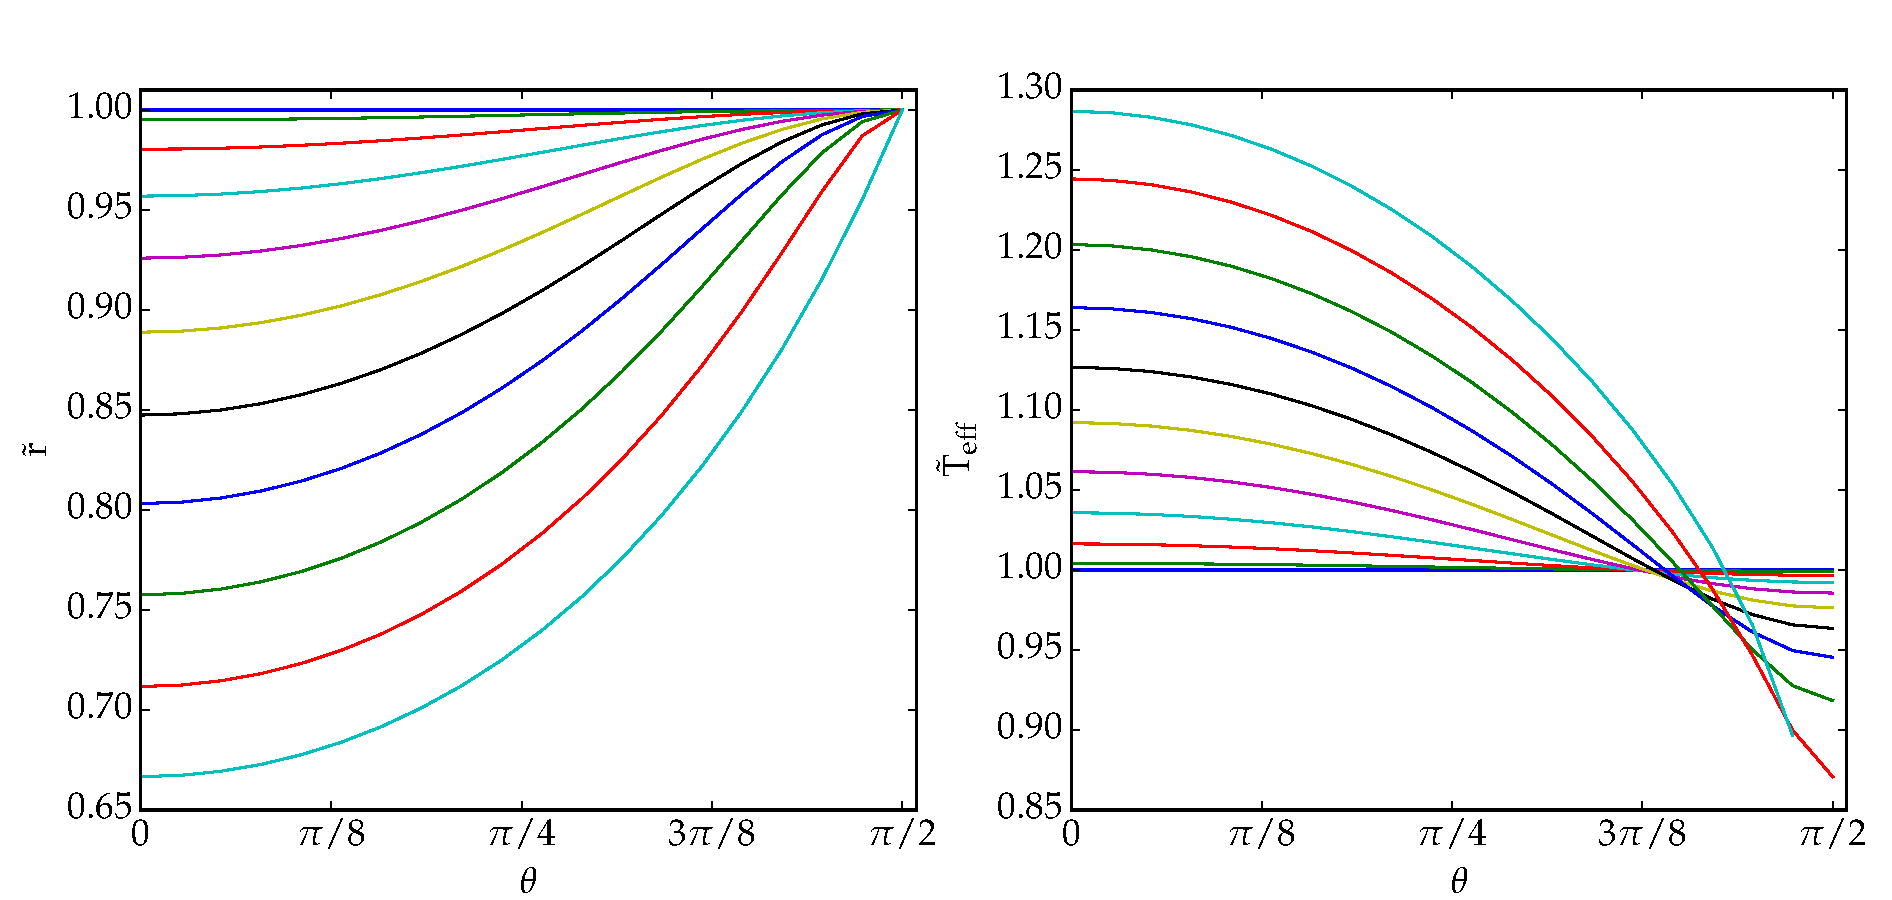
\includegraphics[width=0.9\textwidth]{../plots/R_and_T.pdf}
  \caption{\emph{Left:} The ratio of the stellar radius to the equatorial radius ($\tilde{r}=R/R_e$) as a function of the polar angle $\theta$ for different values of $\omega$. \emph{Right:} Similar to the left panel but now showing the scaled $\tilde{\Teff}$ variable of ELR, see text for details.\label{fig:ELR}}
\end{figure}

Figure \ref{fig:ELR} shows the solution of the ELR model as a function of
$\theta$ for different values of $\omega$. Figure \ref{fig:ELR} indicates
that the polar radius varies from $R_p = R_e$ ($\omega=0$) to $R_p = (2/3) R_e$
($\omega=\pi/2$).


\section{Oblate spheroids and projection effects}
Now that we have a solution for the scaled flux ($\tilde{F}$) we can
compute the projected luminosity along the line of sight (LOS). The surface is
an oblate spheroid so we work in oblate spheroidal coordinates. The coordinate
system is defined by three variables: polar angle $\nu$, azimuthal angle
$\phi$, and $\mu$ = $arctanh( R_p /R_e )$. It is important to distinguish
between $\nu$ in the oblate spheroidal coordinate system and the polar angle
$\theta$ in the ELR model: $\nu = 0$ at the equator; $\nu = \pi/2$ at the pole
and, thus, $\theta = \pi/2 - \nu$.

With the oblate spheroidal coordinate system thus defined, and properly
connected to the ELR model, we can now integrate over the stellar surface
$\Sigma$. However, the quantity that we want is that projected along the line
of sight (LOS) and for that we need to define one additional angle $i$ and the
LOS unit vector $\hat{l}$. $i$ is chosen such that $i = 0$ at the equator.
The projected surface is denoted by $\Sigma_{proj}$.

A useful analytical formula to calculate $\Sigma_{proj}$ is given by
Binngeli~(1980). Note that Brandt \& Huang (2015) use a different formula,
which is only (trivially) correct at $i = 0$ and $\pi/2$. The Brandt \& Huang
formula leads to a maximum error of $\sim8\%$ in $\Sigma_{proj}$ at $i = \pi/4$.

To calculate the luminosity projected along the LOS $L_{proj}$ requires the
surface integral
\begin{equation}
  L_{proj} = 4 \iint \limits_{d\vec{\Sigma} \cdot \hat{l} > 0} F d\vec{\Sigma} \cdot \hat{l}
\end{equation}
where only the flux projected toward the observer, i.e., $d\vec{\Sigma} \cdot \hat{l} \geq 0$, is kept. Once $L_{proj}$ and $\Sigma_{proj}$ are known, the projected effective temperature, $\Teff_{proj}$, can be obtained from the Stefan-Boltzmann law
\begin{equation}
\Teff_{proj} = \left( \frac{L_{proj}}{\sigma \Sigma_{proj}} \right)^{1/4}
\end{equation}
where $\sigma$ is the Stefan-Boltzmann constant.

The following is based closely on what is done in the SYCLIST code
(Georgy et al.\ 2014, A\&A, 566, 21). The double integral (4) is, essentially, a
geometric factor that does not depend on the stellar temperature or luminosity.
It only depends upon $\omega$ and $i$. Thus, it makes sense to derive correction
factors which allow the projected quantities to be determined from the model
intrinsic quantities by geometric scaling factors, i.e.,
\begin{equation}
  L_{proj}(\omega,i) = C_L(\omega,i) L
\end{equation}
and
\begin{equation}
  \Teff_{proj}(\omega,i) = C_T(\omega,i) \Teff
\end{equation}
Thus defined, the geometric factors $C_L$ and $C_T$ are given by
\begin{equation}
C_L = \frac{4 \iint\limits_{d\Sigma \cdot l > 0} F \vec{d\Sigma} \cdot \hat{l} }{\iint\limits_\Sigma F d\Sigma}
\end{equation}
and
\begin{equation}
C_T = \left( \frac{C_L \Sigma}{4 \Sigma_{proj}} \right)^{1/4}
\end{equation}

\begin{figure}
  \centering
  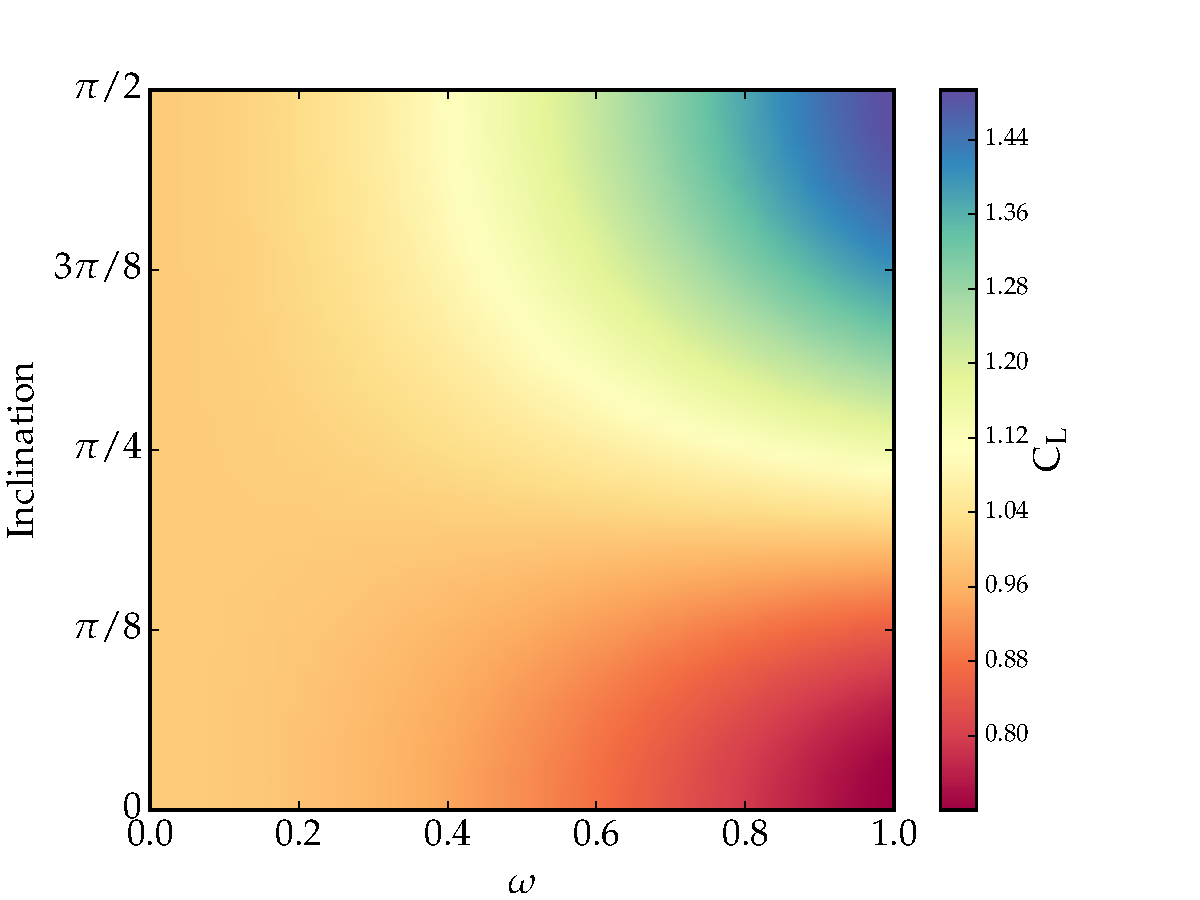
\includegraphics[width=0.9\textwidth]{../plots/C_L.pdf}
  
  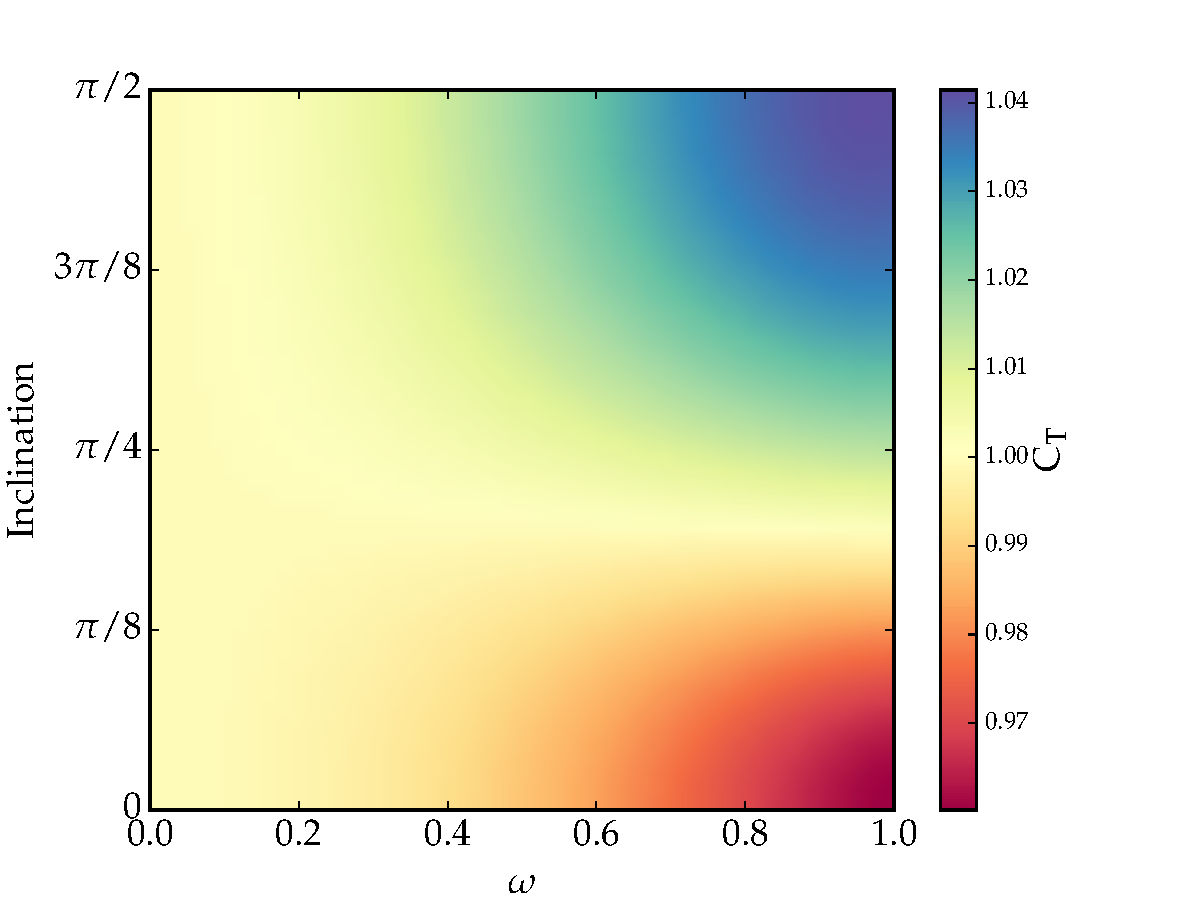
\includegraphics[width=0.9\textwidth]{../plots/C_T.pdf}
  
  \caption{The range of $C_L$ (upper panel) and $C_T$ (lower panel). Note the
    color scale is different in the two panels. \label{fig:coeff}}
\end{figure}

Figure \ref{fig:coeff} shows how the values of $C_T$ and $C_L$ vary over the
$omega$,$i$-plane. These can be compared with the upper panels of Figure XXX
in Georgy et al.\ (2014). The variation in $C_L$ is greater than that of $C_T$
due to the 1/4-power relationship between the two. At $\omega=1$, where
the geometric factors change the most, $C_L$ varies from $-25\%$ to
$+50\%$ while $C_T$ varies by $\pm4\%$. When the LOS is oriented at
$i=34^{\circ}$ ($0.6$ rad) above the equatorial plane, both $C_L~,~C_T \simeq 1$
for all $\omega$.

\section{Python code for $C_T$ and $C_L$}
The github repository provides Python code to numerically solve the differential equations in the ELR model
and to compute the geometric coefficients $C_L$ and $C_T$ for arbitrary $\omega$ and $i$. The repository
also includes a Python interface to interpolate $C_L$ and $C_T$ coefficients from a $50\times50$ grid
stored in a data file.  Separate interpolants are provided for $C_L$ and $C_T$ to enable the application
of gravity darkening corrections to stellar evolution models. As an example, Figure \ref{fig:HRD} shows
a MIST isochrone (Choi et al.\ 2016, ApJ, 823, 102) with $\omega=0.4$ (at the ZAMS). The figure shows the
intrinsic model quantities as well as the gravity-darkened values at $i=0$ (``edge-on'') and $i=90^{\circ}$
(``face-on'').


\end{document}
